\chapter{Klassische Skalierungsmethoden}

    \section{Pixel-Verdopplung}

        \begin{figure}[h]
            \centering
            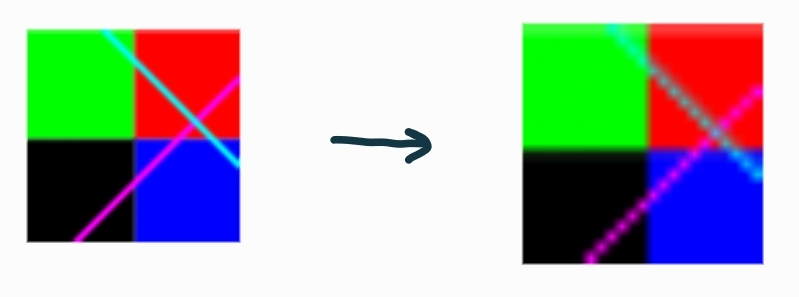
\includegraphics[width=0.6\textwidth]{img/so_sieht_pixel_verdopplung_aus.jpg}
            \caption{Beispielhafte Darstellung einer Skalierung durch PixelVerdopplung}
            \label{fig:beispielhafte_darstellung_einer_skalierung_durch_pixelverdopplung}
        \end{figure}

        Die Pixel-Verdopplung vergrößert das Bild, indem jeder Pixel dupliziert wird.
        Diese Methode kann schnell und einfach umgesetzt werden, indem jeder Pixelwert einfach auf den Nachbarpixel übertragen wird.
        Wenn Bilder mit dieser Methode stark vergrößert werden, ergeben sich oft pixelige und unscharfe Ausgaben, da die Details nicht wirklich vorhanden sind, sondern nur durch die Duplizierung von Pixeln aufgefüllt werden. 
        Aus diesem Grund wird Pixel-Verdopplung oft als eine minderwertige Skalierungsmethode betrachtet und findet in professionellen Anwendungen selten Gebrauch.~\footfullcite{WANG1983363}


    \newpage
    Eine beispielhafte Implementierung in Python sieht folgendermaßen aus:
    
    \begin{lstlisting}[caption={Python-Klasse zur Pixelverdopplung und Bildmanipulation: Implementierung des Algorithmus mit der Pillow-Bibliothek und Erklärung des Codes von PixelVerdopplung: \url{https://github.com/studienarbeit-cnn-dhbwka-2022/Code/blob/main/backend/skalierungsmethoden/pixel_verdopplung.py}.}]
    class PixelVerdopplung(Image):
        def __init__(self, path):
            extend = "p2"
            super().__init__(path, extend)
        
        def manipulate(self, new_size):
            super().manipulate(new_size)
        
            for y in range(self.new_height):
                for x in range(self.new_width):
                    x_old = int(x / (self.new_width / self.width))
                    y_old = int(y / (self.new_height / self.height))
        
                    # Check that x_old and y_old are within bounds of original image
                    if x_old >= self.width:
                        x_old = self.width - 1
                    if y_old >= self.height:
                        y_old = self.height - 1
        
                    old_pixel = self.img.getpixel((x_old, y_old))
                    self.newImg.putpixel((x, y), old_pixel)
        
            return self.save()
    \end{lstlisting}
        
        Die vorliegende Implementierung in Python beschreibt die Realisierung der Pixelverdopplungsklasse, welche in der Lage ist, ein größeres Bild zu erzeugen, indem die leeren Pixel mit demselben Pixelwert wie der nächste Nachbarpixel befüllt werden.
        Der Code ist darauf ausgelegt, eine einfache Möglichkeit bereitzustellen, um ein Bild auf eine höhere Auflösung zu skalieren, wodurch fehlende Details ausgeglichen werden können.
        Dabei wird eine lineare Interpolation auf der Basis der Nachbarpixel durchgeführt, um das neue Bild zu generieren.
        Die Klasse "PixelVerdopplung" erbt von der Klasse "Image" und besitzt einen Konstruktor, der den Pfad zum Bild und die Erweiterung "p2" als Argumente erhält. 
        Die Methode "manipulate" ist dafür zuständig, das Bild auf die gewünschte Größe zu skalieren und zu manipulieren.
        Innerhalb der Methode werden Schleifen durchlaufen, um jeden neuen Pixel im manipulierten Bild zu generieren. 
        Die Koordinaten des jeweiligen alten Pixels werden durch Division der neuen Koordinaten durch die Skalierungsfaktoren berechnet und auf den nächstgelegenen Integer gerundet.
        Um sicherzustellen, dass die berechneten Koordinaten innerhalb der Grenzen des ursprünglichen Bildes liegen, werden sie in einem nächsten Schritt auf den maximalen Index des Bildes zurückgesetzt, falls sie außerhalb liegen sollten. 
        Anschließend wird der Pixelwert des entsprechenden alten Pixels abgerufen und als neuer Pixel an der berechneten Stelle im neuen Bild platziert.
        Die Implementierung dieses Algorithmus stellt eine einfache Möglichkeit dar, um ein Bild auf eine höhere Auflösung zu skalieren, wodurch ein besseres visuelles Ergebnis erzielt werden kann. 
        Dabei ist darauf zu achten, dass die lineare Interpolation eine höhere Laufzeit und Speicheranforderungen aufweist als andere Interpolationsmethoden.
        
    \section{Nearest-Neighbor-Interpolation}
        Die Nearest-Neighbor-Interpolation ist eine weitere Methode zur Skalierung von Bildern. 
        Es wird für jedes Pixel im Ausgabebild der am nächsten liegende Pixel im Eingabebild ausgewählt und der Farbwert des ausgewählten Pixels wird als Farbwert des entsprechenden Pixels im Ausgabebild verwendet.
        Die Verwendung von Nearest-Neighbor-Interpolation ist einfach und schnell zu implementieren. 
        Aufgrund ihrer geringen Komplexität ist sie daher sehr beliebt. 
        Die Methode eignet sich besonders gut für die Vergrößerung von Bildern mit großen, einheitlichen Bereichen oder harten Kanten. 
        

        \begin{acronym}
          \acro{NNI}{Nearest Neighbor Interpolation}
        \end{acronym}
        \begin{lstlisting}
        import numpy as np
        import cv2
        
        def nearest_neighbor_interpolation(image, scale_factor):
            new_size = (int(image.shape[1] * scale_factor), int(image.shape[0] * scale_factor))
            
            scaled_image = np.zeros(new_size + (image.shape[2],), dtype=np.uint8)
            for i in range(new_size[0]):
                for j in range(new_size[1]):
                    x = int(i / scale_factor)
                    y = int(j / scale_factor)
                    scaled_image[j, i] = image[y, x]
            
            return scaled_image
        
        
        image = cv2.imread('example_image.jpg')
        scaled_image = nearest_neighbor_interpolation(image, 2)
        cv2.imshow(image)
        cv2.imshow(scaled_image)
        \end{lstlisting}\footfullcite{jiang2015quantum}
        %TODO @Marc kannst du mir ne Schöne Grafik machen, wo du diesen Code kurz über unser Beispielbild laufen lässt und wir so nen rechts/links Vergleich haben?

        Bei der Verkleinerung von Bildern erleiden diese jedoch oft einen Qualitätsverlust.
        Hier kommt es zu Unschärfe und Blockbildung.
        Dieser Effekt verstärkt sich, wenn das Verhältniss zwischen Quellbild und Audgabebild kein Vielfaches ist.

    \section{Bilineare Interpolation}
    
    % Interpolation cool weil, schnell und ergebniss recht schön.

    % Bilinear ist well aus 2 pixel linear interpoliert wird. (Bild farbig)
    % Die Distanz wir linear berechnet aus den 4 nachbar pixel (Graph 2 punkte)
    % wird fast überall genutzt (citation und quelle angeben)
    
    % Vorteile: Schnell und kompilizert zu programmieren, sieht nicht beschissen aus und kann immer angewendet werden
    % Nachteile: Sieht nicht perfekt aus (Siehe Bicubic oder lanzeros) - ist bei extremen skalierungen nicht super

        Die bilineare Interpolation ist eine weit verbreitete Methode zur Skalierung von Bildern.
        Sie basiert auf dem Konzept der linearen Interpolation und wird häufig in Grafikanwendungen und Bildverarbeitungsalgorithmen eingesetzt.
        Bei der bilinearen Interpolation werden zwei Pixelwerte linear interpoliert, um den Wert eines Zwischenpunkts zu berechnen.
        Dieser Ansatz führt zu einer relativ schnellen Berechnung und liefert ästhetisch ansprechende Ergebnisse.

        \begin{figure}[h]
            \centering
            
\includegraphics[width=0.5\textwidth]{img/so_sieht_bilineare_verdopplung_aus}
            \caption{So sieht bilineare Verdopplung aus.}
            \label{fig:so_sieht_bilineare_verdopplung_aus}
        \end{figure}

        Der Prozess der bilinearen Interpolation bezieht sich auf die Berechnung der Distanz zwischen dem zu interpolierenden Punkt und den umliegenden vier Pixeln.
        Diese Distanz wird linear verwendet, um gewichtete Durchschnittswerte der umgebenden Pixel zu erzeugen.
        Dieser Ansatz ermöglicht eine glattere Darstellung von Zwischenwerten im Vergleich zu einfacheren Interpolationsmethoden wie der nächsten Nachbar-Interpolation.


        \begin{figure}[h]
            \centering
            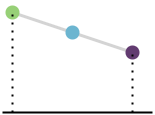
\includegraphics[width=0.5\textwidth]{img/pixel_verdopplung_graph.png}
            \caption{Graph über bilineare Skalierung.}
            \label{fig:graph_uber_bilineare_skalierung}
        \end{figure}

        Die bilineare Interpolation wird aufgrund ihrer Einfachheit und Effizienz häufig eingesetzt.
        Sie ist schnell zu implementieren und kann auf unterschiedliche Bildgrößen angewendet werden.
        Viele Bildbearbeitungssoftware und Grafikbibliotheken nutzen bilineare Interpolation als Standardmethode für die Skalierung von Bildern.
        Dennoch hat die bilineare Interpolation einige Nachteile, insbesondere bei extremen Skalierungen.
        Bei sehr großen oder kleinen Skalierungsfaktoren können Artefakte auftreten, die zu einer verminderten Bildqualität führen.
        In solchen Fällen können fortgeschrittenere Interpolationsverfahren wie Bicubic oder Lanczos eine bessere Wahl sein.


    \begin{figure}[h]
        \centering
        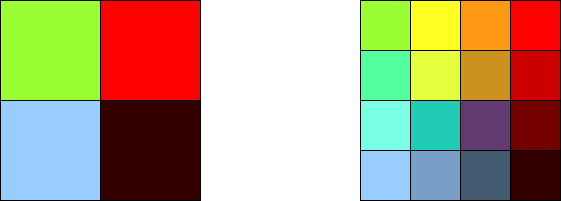
\includegraphics[width=0.5\textwidth]{img/pixel_verdopplung.png}
        \caption{Beispielgrafik zur Pixelverdopplung.}
        \label{fig:beispielgrafik_zur_pixelverdopplung}
    \end{figure}
    
    
    \begin{lstlisting}
    for y in range(self.new_height):
        for x in range(self.new_width):
            x_old = x / (self.new_width / self.width)
            y_old = y / (self.new_height / self.height)
    
            # Find the surrounding pixels
            x1 = int(x_old)
            x2 = min(x1 + 1, self.width - 1)
            y1 = int(y_old)
            y2 = min(y1 + 1, self.height - 1)
    
            # Check if x2 and y2 are out of bounds, if they are substract one
            if x2 == self.width - 1:
                x2 = x1
                x1 -= 1
            if y2 == self.height - 1:
                y2 = y1
                y1 -= 1
    
            # Find the weights
            w1 = (x2 - x_old) * (y2 - y_old)
            w2 = (x_old - x1) * (y2 - y_old)
            w3 = (x2 - x_old) * (y_old - y1)
            w4 = (x_old - x1) * (y_old - y1)
    
            # Get the pixel values of the surrounding pixels
            p1 = self.img.getpixel((x1, y1))
            p2 = self.img.getpixel((x2, y1))
            p3 = self.img.getpixel((x1, y2))
            p4 = self.img.getpixel((x2, y2))
    
            # Interpolate the pixel value
            new_pixel = (
                int(w1 * p1[0] + w2 * p2[0] + w3 * p3[0] + w4 * p4[0]),
                int(w1 * p1[1] + w2 * p2[1] + w3 * p3[1] + w4 * p4[1]),
                int(w1 * p1[2] + w2 * p2[2] + w3 * p3[2] + w4 * p4[2])
            )
            self.newImg.putpixel((x, y), new_pixel)
    \end{lstlisting}\footfullcite{1409828}
    
\section{Bikubische Interpolation}

\subsection{Mathematische Grundlagen}


% Erläuterung der mathematischen Grundlagen der bikubischen Interpolation, einschließlich der Verwendung von kubischen Polynomen und der Stichprobentheorie.
% Herleitung der bikubischen Interpolationsformel und der Eigenschaften der resultierenden Funktion.
% Diskussion der Vor- und Nachteile der Verwendung kubischer Funktionen für die Interpolation im Vergleich zu anderen Funktionstypen.
% Überblick über die Rolle der Fourier-Analyse und der Fourier-Transformationen bei der Bildinterpolation und wie sich dies auf die bikubische Interpolation bezieht.
    
Die bikubische Interpolation ist ein mathematisches Verfahren zur Schätzung der Werte einer kontinuierlichen Funktion an einer gegebenen Stelle, indem eine Funktion mit kubischen Polynomen verwendet wird, die durch benachbarte Funktionswerte verläuft.
Dabei wird das umliegende Gebiet untersucht und die Werte werden basierend auf der Stichprobentheorie geschätzt.

Die bikubische Interpolationsformel ist eine Erweiterung der Bilinearinterpolation auf vier umliegende Pixel und verwendet eine Funktion, die durch benachbarte Funktionswerte verläuft.
Die resultierende Funktion ist stetig differenzierbar und besitzt glatte partielle Ableitungen.

\begin{figure}[h]
    \centering
    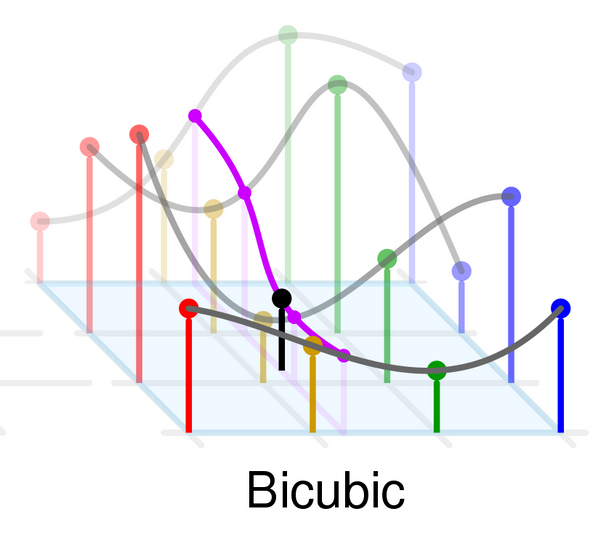
\includegraphics[width=0.5\textwidth]{img/bicubic_graph}
    \caption{Bikubische Interpolation}
    \label{fig:bicubic_interpolation}
\end{figure}

Im Vergleich zu anderen Interpolationsverfahren wie der bilinearen Interpolation und der Lanczos-Interpolation hat die bikubische Interpolation den Vorteil, dass sie eine höhere Genauigkeit bei der Schätzung von Pixelwerten bietet.
Ein Nachteil ist jedoch, dass sie im Allgemeinen höhere Rechenaufwendungen erfordert.

Die Fourier-Analyse und die Fourier-Transformationen spielen eine wichtige Rolle bei der Bildinterpolation, da sie es ermöglichen, die Funktion in den Frequenzraum zu transformieren und damit eine effektivere Interpolation zu erreichen.

\subsection{Algorithmische Implementierung}


% Überblick über die algorithmischen Schritte bei der bikubischen Interpolation, einschließlich der Auswahl der umgebenden Pixel und der Gewichte sowie der Berechnung der neuen Pixelwerte.
% Diskussion von Techniken zur Optimierung der Leistung der bikubischen Interpolation, wie z. B. die Vorberechnung von Lookup-Tabellen, Parallelisierung und Speicherverwaltung.
% Untersuchung von Grenzfällen und Randbedingungen, die bei der bikubischen Interpolation auftreten können, und wie diese effektiv behandelt werden können.
% Vergleich der algorithmischen Implementierung der bikubischen Interpolation mit anderen Interpolationsverfahren, wie z.B. der bilinearen Interpolation und der Lanczos-Interpolation.

    
Die bikubische Interpolation erfolgt durch die Auswahl von umgebenden Pixeln und deren Gewichte sowie der Berechnung der neuen Pixelwerte.

Sie verwendet eine 4x4-Matrix umliegender Pixel, um den Wert an einem bestimmten Punkt zu berechnen.
Die Formel zur Berechnung lautet:

Die Koeffizienten $a_{ij}$ werden basierend auf den umliegenden Pixelwerten und ihren Ableitungen berechnet.
Dieses Verfahren ermöglicht eine glatte Interpolation zwischen den Pixeln und hinterlasst wenige scharfe Kanten.

\begin{equation}
    f(x,y) = \sum_{i=0}^{3}\sum_{j=0}^{3}a_{i,j}*x^{i}*y^{j}
\end{equation}

Eine Möglichkeit zur Optimierung der Leistung besteht darin, Lookup-Tabellen vorzubereiten, Parallelisierungstechniken zu verwenden und die Speicherverwaltung zu optimieren.
Grenzfälle und Randbedingungen können bei der bikubischen Interpolation auftreten und müssen effektiv behandelt werden.
Die algorithmische Implementierung der bikubischen Interpolation kann mit anderen Interpolationsverfahren wie der bilinearen Interpolation und der Lanczos-Interpolation verglichen werden.

Die Koeffizienten $a_{ij}$ werden basierend auf den umliegenden Pixelwerten und ihren Ableitungen berechnet.
Dieses Verfahren ermöglicht eine glatte Interpolation zwischen den Pixeln und hinterlasst wenige scharfe Kanten.

Die Methode `manipulate` der Klasse `BicubicInterpolation` implementiert die bikubische Interpolation für das Vergrößern von Bildern.
Der wichtigste Teil des Codes ist die Schleife, die über jedes Pixel einen Kernel berechnet, der die jeweiligen Gewichte der benachbarten Pixel erechnet.
In den genannten Zeilen wird ein 4x4-Kern um das aktuelle Pixel herum gebildet und für jeden Pixel im Kern werden die Gewichte berechnet.
Dabei wird die `\_get\_weight`-Funktion aufgerufen, welche auf der Basis einer kubischen Kurve das Gewicht für einen bestimmten Abstand berechnet.
Die berechneten Gewichte werden in eine Liste `weights` hinzugefügt.
Diese Gewichte dienen später bei der Interpolation des aktuellen Pixels als multiplikative Faktoren für die umliegenden Pixel im Originalbild.

Eine Möglichkeit zur Optimierung der Leistung besteht darin, Lookup-Tabellen vorzubereiten, Parallelisierungstechniken zu verwenden und die Speicherverwaltung zu optimieren.
Grenzfälle und Randbedingungen können bei der bikubischen Interpolation auftreten und müssen effektiv behandelt werden.
Die algorithmische Implementierung der bikubischen Interpolation kann mit anderen Interpolationsverfahren wie der bilinearen Interpolation und der Lanczos-Interpolation verglichen werden.

Unsere Implementierung der bikubischen Interpolation in Python ist im Abschnitt \ref{sec:bicubic-implementation}.

\subsection{Analyse der Leistung}

    Zur Bewertung der Leistung von Bildinterpolationsverfahren werden verschiedene Kriterien verwendet, einschließlich der visuellen Qualität, der Genauigkeit und der Berechnungseffizienz. 
    Die Leistung der bikubischen Interpolation kann mit anderen Interpolationstechniken anhand von Testbildern und Datensätzen verglichen werden. 
    Dabei werden verschiedene Parameter wie Bildgröße, Auflösung und Inhalt untersucht, um ihre Auswirkungen auf die Leistung der bikubischen Interpolation zu analysieren.

    \subsection{Implementation}\label{sec:bicubic-implementation}
    \begin{lstlisting}[caption={Python-Klasse zur Bikubischen interpolation \url{https://github.com/studienarbeit-cnn-dhbwka-2022/Code/blob/main/backend/skalierungsmethoden/bicubic_interpolation.py}.}]
import math
from backend.image import Image

def _cubic(x, a=-0.5):
    abs_x = abs(x)
    if abs_x <= 1:
        return (a + 2) * (abs_x ** 3) - (a + 3) * (abs_x ** 2) + 1
    elif abs_x < 2:
        return a * (abs_x ** 3) - (5 * a) * (abs_x ** 2) + (8 * a) *
abs_x - (4 * a)
    return 0

    \subsection{Implementation}
    \begin{lstlisting}
import math
from backend.image import Image

def _cubic(x, a=-0.5):
    abs_x = abs(x)
    if abs_x <= 1:
        return (a + 2) * (abs_x ** 3) - (a + 3) * (abs_x ** 2) + 1
    elif abs_x < 2:
        return a * (abs_x ** 3) - (5 * a) * (abs_x ** 2) + (8 * a) *
abs_x - (4 * a)
    return 0

def _get_weight(distance):
    abs_distance = abs(distance)
    if abs_distance <= 1:
        return _cubic(abs_distance)
    return 0

class BicubicInterpolation(Image):
    def __init__(self, path):
        extend = "biCu"
        super().__init__(path, extend)

    def manipulate(self, new_size):
        super().manipulate(new_size)

        for y in range(self.new_height):
            for x in range(self.new_width):
                px = x * self.width / self.new_width
                py = y * self.height / self.new_height

                ix = math.floor(px)
                iy = math.floor(py)

                dx = px - ix
                dy = py - iy

                weights = []
                for j in range(-1, 3):
                    for i in range(-1, 3):
                        weight = _get_weight(i - dx) * _get_weight(dy - j)
                        weights.append(weight)

                total_weight = sum(weights)
                normalized_weights = [w / total_weight for w in weights]

                new_pixel = [0, 0, 0]
                for j in range(-1, 3):
                    for i in range(-1, 3):
                        ox = ix + i
                        oy = iy + j
                        if ox < 0 or oy < 0 or ox >= self.width or
oy >= self.height:
                            pixel_value = list(
                                self.img.getpixel((min(max(ox, 0),
self.width - 1), min(max(oy, 0), self.height - 1)))
                            )
                        else:
                            pixel_value = list(self.img.getpixel(
(ox, oy)))

                        weight_index = (j + 1) * 4 + (i + 1)
                        weight = normalized_weights[weight_index]
                        for k in range(3):
                            new_pixel[k] += weight * pixel_value[k]

                self.newImg.putpixel((x, y), (int(new_pixel[0]),
int(new_pixel[1]), int(new_pixel[2])))

        return self.save()
    \end{lstlisting}
    
    Die Methode `manipulate` der Klasse `BicubicInterpolation` implementiert die bikubische Interpolation für das Vergrößern von Bildern.
    Der wichtigste Teil des Codes ist die Schleife, die über jedes Pixel einen Kernel berechnet, der die jeweiligen Gewichte der benachbarten Pixel erechnet.
    In den genannten Zeilen wird ein 4x4-Kern um das aktuelle Pixel herum gebildet und für jeden Pixel im Kern werden die Gewichte berechnet.
    Dabei wird die `\_get\_weight`-Funktion aufgerufen, welche auf der Basis einer kubischen Kurve das Gewicht für einen bestimmten Abstand berechnet.
    Die berechneten Gewichte werden in eine Liste `weights` hinzugefügt.
    Diese Gewichte dienen später bei der Interpolation des aktuellen Pixels als multiplikative Faktoren für die umliegenden Pixel im Originalbild.
    
    \subsection{Anwendungen}

Die bikubische Interpolation wird in verschiedenen Anwendungen der Bildverarbeitung eingesetzt und bietet bestimmte Vorteile gegenüber der bilinearen Interpolation.
Ein Bereich, in dem die bikubische Interpolation besser geeignet sein kann, ist die Bildskalierung und -größenänderung.
Durch die Verwendung von zusätzlichen benachbarten Pixeln in der Interpolationsmethode kann die bikubische Interpolation feinere Details beibehalten und glattere Übergänge erzeugen, was zu hochwertigeren skalierten Bildern führen kann.

Ein weiterer Anwendungsbereich ist die Bildrotation und -transformation.
Bei der bikubischen Interpolation werden nicht nur benachbarte Pixel, sondern auch deren benachbarte Pixel berücksichtigt, wodurch eine bessere Anpassung an die gewünschten Rotationen oder Transformationen ermöglicht wird.
Dies kann zu weniger Verzerrungen und einem insgesamt realistischeren Ergebnis führen.

Die bikubische Interpolation kann auch in der Bildentrauschung und -wiederherstellung nützlich sein.
Durch die Verwendung von zusätzlichen Pixeln und einer gewichteten Interpolation können Rauschanteile reduziert und verloren gegangene Informationen wiederhergestellt werden.
Dies kann insbesondere in der medizinischen Bildgebung und der Satellitenbildgebung von Vorteil sein, wo genaue und zuverlässige Bilder erforderlich sind.

Wichtig zu beachten ist, dass die Eignung der bikubischen Interpolation von verschiedenen Faktoren abhängt, einschließlich der Natur des Eingangsbildes, des gewünschten Ausgabekontexts und der verfügbaren Rechenleistung.
In einigen Fällen kann die bikubische Interpolation aufgrund ihrer erhöhten Berechnungskosten und möglichen Unschärfen weniger geeignet sein.
Eine sorgfältige Bewertung der spezifischen Anforderungen und der verfügbaren Optionen ist daher umso entscheidender, um die optimale Interpolationsmethode für eine bestimmte Anwendung zu bestimmen.

    \subsection{Erweiterungen und Variationen}

    Erläuterung der verschiedenen Erweiterungen und Variationen der bikubischen Interpolation, wie z.
    B. Super-Resolution-Techniken, Multiskalen- und pyramidenbasierte Interpolation und adaptive Interpolationstechniken.
    Diskussion der Vor- und Nachteile dieser Varianten und ihrer Eignung für verschiedene Bildtypen und Anwendungen.
    Erkundung potenzieller künftiger Forschungsrichtungen in diesem Bereich, z.
    B. auf Deep Learning basierende Ansätze, ungleichmäßige und unregelmäßige Abtastverfahren sowie mehrdimensionale und mehrkanalige Interpolation.


\section{Lanczos-Interpolation}
    Die Lanczos-Interpolation ist eine Methode zur Rekonstruktion von Werten im Bild aus diskreten Abtastungen. 
    In diesem Abschnitt wird die mathematische Grundlage und die praktische Anwendung der Lanczos-Interpolation kurz erläutert.

\subsection{Mathematische Grundlage}

    Die Lanczos-Interpolation basiert auf der Idee, ein kontinuierliches Signal $f(x)$ durch eine Summe von gewichteten Basisfunktionen zu approximieren. 
    Dieses Signal können zum Beispiel Farbwerte in einem Bild sein.
    Die Basisfunktionen werden durch das sogenannte Lanczos-Kernel definiert:

\begin{equation}
    L(x) = \begin{cases} \frac{a \cdot \sin(\pi \cdot x) \cdot \sin(\pi \cdot x / a)}{(\pi \cdot x)^2} & \text{wenn } \left| x \right| < a \\ 0 & \text{sonst} \end{cases}
\end{equation}
~\footfullcite{duchon1979lanczos}

Das Lanczos-Kernel hat eine kompakte Trägerfunktion.
Eine kompakte Trägerformel bedeutet, sie ist nur in einem begrenzten Bereich von Null verschieden. 
In der Praxis hat dies den Vorteil, dass das Signalrauschen in Bereichen außerhalb des Bereichs im Signalraum reduziert wird und somit eine bessere Interpolation des Signals erreicht werden kann.
Die Gewichtungen der Basisfunktionen werden durch die Interpolationskoeffizienten bestimmt, die durch die diskreten Abtastungen des Signals berechnet werden.

Die Lanczos-Interpolation wird in der Regel auf gleichmäßig verteilten Stützstellen angewendet. 
Die Interpolationsmethode verwendet diese Stützstellen als Ausgangspunkt, um eine Schätzung des Signals an anderen Orten zu berechnen. 
Seien $x_1, x_2, \ldots, x_n$ die Stützstellen des Signals und $y_1, y_2, \ldots, y_n$ die zugehörigen Abtastungen.
Die Interpolationsfunktion $s(x)$ kann dann wie folgt berechnet werden:

\begin{equation}
    s(x) = \sum_{i=1}^{n} y_i \cdot L(x - x_i)
\end{equation}

Hierbei ist $L(x - x_i)$ die Lanczos-Kernel-Funktion, die den Beitrag des i-ten Stützpunkts zum interpolierten Signal an der Position x angibt.
Die Gewichtung erfolgt durch Multiplikation der Abtastung $y_i$ mit dem Wert des Lanczos-Kernels für den Abstand zwischen der Stützstelle $x_i$ und dem Zielpunkt x.

Die Wahl des Parameters $a$ beeinflusst die Schärfe der Interpolation.
Ein kleinerer Wert von $a$ führt zu einer breiteren Trägerfunktion und einer glatteren Interpolation, während ein größerer Wert von $a$ zu einer schärferen Trägerfunktion und einer detailreicheren Interpolation führt.
Es ist wichtig zu beachten, dass bei zu großen Werten von $a$ sogenannte Ringing-Artefakte auftreten können, bei denen sich unerwünschte Oszillationen um Kanten oder Kontrastübergänge im Bild bilden.

Insgesamt bietet die Lanczos-Interpolation eine effektive Methode zur Skalierung von Bildern mit Erhaltung von Details und Schärfe.
Sie ist jedoch rechenaufwändiger als einfachere Interpolationsmethoden, da sie eine Berechnung für jeden Pixel im skalierten Bild erfordert.
~\footfullcite{BENTBIB2016233}

\subsection{Praktische Anwendung}

Die Lanczos-Interpolation findet Anwendung in vielen Bereichen der Bildverarbeitung. 
Ein Anwendungsbeispiel ist die Upsampling von digitalen Bildern, um eine höhere Auflösung zu erreichen.

Die praktische Umsetzung der Lanczos-Interpolation erfordert die Berechnung der Interpolationskoeffizienten und die Bestimmung der Stützstellen des Signals. 
In der Regel werden hierfür spezielle Algorithmen eingesetzt, die auf der effizienten Berechnung der Basisfunktionen basieren.

\begin{lstlisting}
from backend.image import Image
import math

class LanczosInterpolation(Image):
    def __init__(self, path):
        extend = "lcz"
        super().__init__(path, extend)

    def lanczos_kernel(self, x, a=2):
        if x == 0:
            return 1
        elif abs(x) >= a:
            return 0
        else:
            return math.sin(math.pi * x) * math.sin(math.pi * x / a) /
(math.pi ** 2 * x ** 2)

    def manipulate(self, new_size):
        super().manipulate(new_size)

        for i in range(self.new_width):
            for j in range(self.new_height):
                x, y = i * self.width / self.new_width, j *
self.height / self.new_height
                u, v = math.floor(x), math.floor(y)
                s, t = x - u, y - v

                pixel = (0, 0, 0)
                weight_sum = 0

                for m in range(u - 2, u + 3):
                    for n in range(v - 2, v + 3):
                        if 0 <= m < self.width and 0 <= n < self.height:
                            weight = self.lanczos_kernel(s - (m - u)) *
self.lanczos_kernel(t - (n - v))
                            pixel = tuple([p + weight * self.img.getpixel(
(m, n))[i] for i, p in enumerate(pixel)])
                            weight_sum += weight
                if weight_sum > 0:
                    pixel = tuple([int(p / weight_sum) for p in pixel])
                    self.newImg.putpixel((i, j), pixel)

        return self.save()
\end{lstlisting}

\section{Zusammenfassung zu Vor- und Nachteilen von Techniken in der Bildverarbeitung}

In der Bildverarbeitung gibt es verschiedene Techniken, die verwendet werden können, um ein Bild zu bearbeiten oder zu manipulieren. 
In diesem Abschnitt werden wir uns mit einigen gängigen Techniken zur Interpolation von Bildern beschäftigen, nämlich Pixelverdopplung, Nearest Neighbour Interpolation, Bilineare Interpolation, Bikubische Interpolation und Lanczos Interpolation. 
Wir werden jeweils auf die Vor- und Nachteile dieser Techniken eingehen.

\subsection{Pixelverdopplung}

Bei der Pixelverdopplung wird jedes Pixel im Bild einfach dupliziert, um ein größeres Bild zu erzeugen. 
Diese Methode ist einfach und schnell, aber sie führt oft zu einer Verzerrung des Bildes und kann zu einer verschlechterten Bildqualität führen.

\subsection{Nearest Neighbour Interpolation}

Die Nearest Neighbour Interpolation ist eine einfache Interpolationsmethode, bei der jeder neue Pixelwert durch den nächstgelegenen Pixelwert im Originalbild bestimmt wird. 
Diese Methode ist einfach und schnell, aber sie führt oft zu einem "Treppeneffekt" im Bild, da die Pixelwerte nicht kontinuierlich interpoliert werden.

\subsection{Bilineare Interpolation}

Die bilineare Interpolation ist eine Methode, bei der die neuen Pixelwerte aus einer bilinearen Funktion berechnet werden, die aus den vier nächstgelegenen Pixeln im Originalbild abgeleitet wird. 
Diese Methode führt oft zu einer glatteren Interpolation als die Nearest Neighbour Interpolation, aber es kann immer noch zu einem "Verwischen" des Bildes kommen.

\subsection{Bikubische Interpolation}

Die bikubische Interpolation ist eine Methode, bei der die neuen Pixelwerte aus einer bikubischen Funktion berechnet werden, die aus den sechzehn nächstgelegenen Pixeln im Originalbild abgeleitet wird.
Diese Methode führt oft zu einer noch glatteren Interpolation als die bilineare Interpolation, aber sie kann auch zu einer Überbetonung von Bildstrukturen führen.

\subsection{Lanczos Interpolation}
Die Lanczos Interpolation ist eine Methode, bei der die neuen Pixelwerte aus einer Lanczos-Funktion berechnet werden, die aus einer begrenzten Anzahl von nächstgelegenen Pixeln im Originalbild abgeleitet wird. 
Diese Methode führt oft zu einer sehr glatten Interpolation und reduziert das Rauschen im Bild, aber sie kann auch zu einer gewissen Unschärfe im Bild führen.

\section{Analyse der Leistung}

    Erläuterung der Kriterien, die zur Bewertung der Leistung von Bildinterpolationsverfahren verwendet werden, einschließlich der visuellen Qualität, der Genauigkeit und der Berechnungseffizienz.

    Untersuchung der Auswirkungen verschiedener Parameter wie Bildgröße, Auflösung und Inhalt auf die Leistung der bikubischen Interpolation.
    Diskussion der potenziellen Einschränkungen und Kompromisse, die mit der Verwendung der bikubischen Interpolation verbunden sind, sowie der Faktoren, die ihre Leistung in verschiedenen Kontexten beeinflussen können.

    \begin{table}[h]
        \begin{tabular}{l|l|l|l}
            Verfahren & Geschwindigkeit & Qualität & Brauchbarkeit \\ \hline \hline
            Nearest Neighbour & schnell & mäßig & blockige Ergebnisse \\ \hline
            Bilineare Interpolation & mittel & gut & linearer Effekt \\ \hline
            Bicubische Interpolation & langsam & sehr gut & glättender Effekt \\ \hline
            Lanczos-Interpolation & langsam & sehr gut & glättender Effekt \\
        \end{tabular}
    \end{table}

Die Beurteilung von Bildinterpolationsverfahren erfolgt anhand diverser Kriterien, welche ihre Leistung charakterisieren.
Zu den frequent verwendeten Kriterien zählen die visuelle Qualität, die Genauigkeit sowie die Berechnungseffizienz.
Die visuelle Qualität bezieht sich auf die subjektive Wahrnehmung der Bildqualität nach der Interpolation.
Wesentliche Aspekte der visuellen Qualität beinhalten die Schärfe der Details, das Vorhandensein von Artefakten (z.B. Unschärfe oder Kantenartefakte) und die allgemeine Ästhetik des interpolierten Bildes.
Die Genauigkeit eines Interpolationsverfahrens betrifft dessen Fähigkeit, die tatsächlichen Werte oder Strukturen des Originalbildes möglichst präzise zu reproduzieren.
Eine präzise Interpolation minimiert den Informationsverlust und wahrt die inhärente Qualität des Bildes.
Die Berechnungseffizienz betrachtet die Laufzeit- und Ressourcenanforderungen des Interpolationsverfahrens.
Zügige und effiziente Methoden ermöglichen eine reibungslose Verarbeitung großer Datenmengen in Echtzeit oder bei der Stapelverarbeitung.

Beispiele aus dem wirklichen Leben umfassen Ladezeiten für Webseiten, medizinische Bildgebung oder Fernerkundung.
In wissenschaftlichen Anwendungen wie der medizinischen Bildgebung oder der Fernerkundung ist es von besonderer Bedeutung, dass präzise Messungen und Analysen durchführbar sind.
Eine präzise Interpolation minimiert den Informationsverlust und wahrt die inhärente Qualität des Bildes.
Die Berechnungseffizienz spielt eine ausschlaggebende Rolle in Anwendungen wie der Videokodierung oder der Echtzeitbildverarbeitung.

Es ist essenziell zu beachten, dass die Leistung der Interpolationsverfahren von diversen Faktoren abhängt, einschließlich der Bildgröße, der Auflösung, des Inhalts und des Kontextes der Anwendung.
Ein Verfahren, welches in einer bestimmten Situation gute Ergebnisse erzielt, kann in einer anderen Situation weniger erfolgreich sein.
Deshalb ist es wichtig, die spezifischen Anforderungen und Beschränkungen einer Anwendung zu berücksichtigen, um das am besten geeignete Interpolationsverfahren auszuwählen.

\subsection{Vergleich und Zusammenfassung}

Insgesamt gibt es keine "beste" Methode zur Interpolation von Bildern, da jede Methode ihre eigenen Vor- und Nachteile hat. 
Die Wahl der Methode hängt von den spezifischen Anforderungen und Einschränkungen ab, die für die jeweilige Anwendung gelten. 
Die Wahl einer geeigneten Interpolationsmethode kann jedoch die Bildqualität erheblich verbessern und zu einer effektiveren Bildverarbeitung führen.
\newpage